\chapter{Time-memory tradeoff}

\paragraph{Summary}


\section{Time-memory tradeoff attack}

\textit{\textbf{Brute force attack.}} A brute force attack on a block cipher would be to try out all the possible keys which could be used to encrypt certain known (or chosen) or unknown plaintext. The key which decrypts the ciphertext to give the known plaintext or most sensible plaintext (if it is unknown) is then the original key. Though very simple in theory, brute force attacks require a very long time to break ciphers in practice. There is no storage required during this attack, but the time required to break the cipher is very long. Though modern computers have advanced tremendously in their computational speed over the last some years, design of new ciphers have incorporated longer key sizes to protect against brute force attacks, making brute forcing even more impractical.

For example, in order to break a 32 bit key, we would need to carry out $2^{32}$ decryptions on available ciphertext. Using a 2GHz processor (which is quite common for personal use), we can run $2^{31}$ clock cycles in one second (as 1 giga is $2^{30}$). Since one encryption would take a fixed number of clock cycles, say a modest $2^3$ cycles, by simple calculation, we can have a brute force attack on the cipher in $2^4$ seconds, or 16 seconds. As can be seen, this is a dismally weak key size. For a key size of 48 bits, the brute-force would take $2^{20}$ seconds which is 1048576 seconds, or just more than 12 days. In modern ciphers, the key sizes starting from 128 bits in length are considered safe. AES uses a minimum key size of 128 bits, which can be extended to use 256 bits. So, just to give a feeling of the security of a 128 bit cipher, it would take an order of $10^{30}$ years to brute force the key.\\

\textit{\textbf{Precomputed ciphertext attack.}} Brute-force attacks are just one side of the coin. The other way of breaking a cipher in a known (or chosen) plaintext attack is to precompute ciphertexts corresponding to all the possible keys and to store the (key, ciphertext) pair in a table in memory. During the attack, the attacker just needs to do a table lookup for the available ciphertext to find the corresponding key. Again, the concept is quite straightforward theoretically, but it also faces the same problem as brute-force attacks, but from a different perspective. A table lookup takes constant time (if efficient hash tables are implemented), so practically the attack time is very less. But, the amount of precomputed data is tremendous and the attacker would need very large amount of memory to save this data for the attack phase. 

Let us take the weaker case of a 32 bit key, which is far from use in today's ciphers. For each of $2^{32}$ possible keys, we need to store 32 bits of key and 32 bits of ciphertext (assuming the plaintext is 32 bits, which could very well be more). This amounts to 64 bits or 8 bytes of data for every possible key. $2^{32}$ such entries would require $2^{32}$ * 8 bytes which is 32 gigabytes. For a random access memory, 32 GB is a high requirement. For higher key sizes, this requirement gets more towards impossible.\\

\textit{\textbf{In between time and memory.}} The technique of time-memory tradeoff is a way between the above two extreme and practically difficult ideas. TMTO solves our problem by using memory in order to reduce the time taken for attack, bringing the requirements for time and memory within  practical domains. As a result, with considerable precomputation, the attack time can be reduced and so are the computational resources required.

Before we go into more details of the working of time-memory tradeoff attacks on ciphers, we would take a simple example of a general application of such tradeoffs. The example has been taken from \cite{stamp2003out}. \\

\textit{\textbf{Simple example.}} Consider the problem of finding the number of \textbf{1}'s in the binary expansion of a non-negative integer $x$ (which takes $4$ bytes). The simplest algorithm to solve this problem would for 32 operations, pick the value of the least significant bit, add it to a global \textit{sum} and shift the integer rightwards by one bit. The \textit{sum} would then be the desired result. The pseudo-code for such an algorithm is shown below.

\begin{verbatim}
// ones_count(x)
sum = 0
for i = 0 to len(x) - 1
    sum = sum + (x >> i) & 1
next i
return sum
\end{verbatim}

Here, $>>$ denotes the right shift operation and \& denotes bitwise binary \emph{and} operation. The algorithm performs 32 operations (based on the length of the integer) and has nearly no memory requirement. The other approach to solve this problem would be to store the required \emph{sum} for each of the possible $2^{32}$ integers in memory. This way, just one memory lookup is required to find the result for $x$. While in this case, we need to have a memory of the order of $2^{32}$. 

One middle way between both these approaches would be to store the \textit{sum} for all possible 8 bit numbers, rather than doing it for all 32 bit numbers. Then the memory required would be of the order of $2^{8}$. Then, we break the 32 bit integer into four bytes, and add the stored \textit{sum} for each of the four bytes, by looking up in the table. If $y_1$, $y_2$, $y_3$ and $y_4$ are the four bytes, such that

\begin{flushleft}
$y_4$ = ($x$ $\&$ $0$xFF)\\
$y_3$ = ($(x >> 8)$ $\&$ $0$xFF)\\ 
$y_2$ = ($(x >> 16)$ $\&$ $0$xFF)\\ 
$y_1$ = ($(x >> 24)$ $\&$ $0$xFF)\\
\end{flushleft}

and if p is the array which stores the \textit{sum} for all possible bytes, then the desired \textit{sum} for $x$ can simply be calculated by

\begin{center}
\large{$sum = p[y_1] + p[y_2] + p[y_3] + p[y_4]$}\\
\end{center}

The number of operations in this case is 4, as there are four lookups made to the precomputed array $p$. This is just one way of realizing a middle way between the parameters of time and memory. If the algorithm stores 4 bit values, with their corresponding \textit{sum}, then the number of operations would be 8. Hence a optimal combination of memory and time can be chosen based on the resources at hand and the application. 

% IMP: do you need to show the table here for different combinations of time and memory? %

\section{Background}
\subsection{Birthday paradox}
\label{sec:bday-paradox}

\textit{\textbf{General birthday paradox.}} Birthday paradox (or birthday problem or surprise, as it is also called), refers to the fact that in a room of 23 people, two people have the same date of birth with a probability greater than one-half. While there are 365 different possible birthdays in a year (excluding the leap year), the birthday paradox looks surprising and non-intuituve at the first glance. But, the figure has been derived from probability theory and is proved. 
% IMP: need a reference here %

A generalized definition of the birthday paradox for can be formulated as follows: given $n$ random integers where each could have $m$ different possible values, the probability that two of them would have the same value is given by the following equation \cite{menezes}.

\begin{center}
\large{$P(m,n)$ $\approx$ $1 - e^{-{n^2}/{2m}}$}
\end{center}

If we replace $m$ by 365, and $n$ by 23 in the above equation, then it can be checked that $P(365,23)$ $\approx$ $0.507$. In addition, $P(365,n)$ rapidly increases as $n$ increases, and the chances of two people having the same birthday becomes nearly $99 \%$ for $n$ = 57. If $m$ is considered to be very large, such that $m \rightarrow \infty$, then the above equation can be reduced, giving us the following condition for chances of nearly $100 \%$. 

\begin{center}
\large{$n$ = $\sqrt{\frac{\pi}{2} \times m}$}
\end{center}

The general birthday paradox is used in cryptography in determining collisions in hash functions. Consider a hash function $H$ with $h$ bits of output. The total number of different outputs the function could produce is $2^{h}$. A collision is said to occur when the hash function produces the same output for two different inputs, i.e. $H(x_1)$ = $H(x_2)$ when $x_1$ $\neq$ $x_2$. Then, according to the birthday paradox, the chances that a collision would occur are close to $100 \%$ after the hash function has produced outputs for $2^{h/2}$ random inputs (if we have $m = 2^h$ and we ignore the factor of $\frac{\pi}{2}$).\\

\textit{\textbf{Variant of the birthday paradox.}} A variant of the birthday paradox (\cite{GeneralizedAttack}) is especially more interesting to us, since it is directly used in TMTO attacks. If we consider two groups of people now instead of just one, then just 17 people are required to be present in each group, so that two people, one from each group, share the same birthday.  

We can generalize the above situation in the following way. We have two groups of random elements each having different number elements, say $n_1$ and $n_2$. The elements are non-negative integers, with both the groups having the same range $m$ for all the integers. According to \cite{menezes}, the probability of at least one coincidence in such a case is given by,
\begin{center}
\large{$P(m, n_1, n_2) = 1 -(1 -\frac{n_2}{m})^{n_1}$}
\end{center}

For the condition that $m \rightarrow \infty$, the above relation is reduced to,
\begin{center}
\large{$P(m, n_1, n_2)$ $\approx$ $1 - e^{-{n_{1} n_{2}}/{m}}$}
\end{center}

For there to be at least one coincidence, the probability must be $1$. Replacing $P(m, n_1, n_2)$ by $1$ and taking the limit $m \rightarrow \infty$, we get the following condition.
\begin{center}
\large{$n_1 \times n_2$ = $\frac{\pi}{4} \times m$ (or)\\}
\large{$n_1 \times n_2 \geq m$}
\end{center}

The last equation above is the birthday paradox we would be using the analysis of most of the TMTO attacks on HiTag2.

% Add the case of handbook statement, with or without replacements?
% also briefly how this paradox would be applied to the TMTO?

% -------------
% what the simple birthday paradox is %

% generalize it in terms of n %

% introduce birthday attack, define scenario (then take hash as example) %

% what is the variant of birthday paradox %

% meet in the middle attack on DES by diffie hellman %
% a TMTO attack would always use variant of birthday attack %

% Question - How can the variant of the birthday problem be derived from the birthday problem?
% Question - Probability of one-half on 23, or is it one? root(pi * m / 2)
% Question - Is meet in the middle attack a TMTO attack? (I think NO!)
% --------------

\subsection{Hash tables}
\label{sec:hash-tables}

Hash tables are used during the precomputation phase as a data structure to store the (prefix, state) pairs in memory. The advantage that hash tables offer is in terms of the search time. The search time provided by hash tables in the best case and the average case is close to $O(1)$, while the worst case search time is $O(n)$ occuring with very less probability. A very important role is played by the hash function chosen for the table. 

The basic data structure for hash tables consists of a pair of data elements, one for holding the \emph{value} to be stored, and the other which acts as a unique identifier for that value, called the \emph{key}. The hast table is basically an array of such (key, value) pairs. Typically in a normal array, pairs would be stored starting from the initial index of the array, with the index increasing with every pair. In a hash table, the pairs are not stored consecutively, but in an order which would make searching them more efficient at a later stage. The index at which a particular pair is stored depends on the key and the hash function. A hash of the key is calculated, and if required, reduced to the domain of the indices. The pair is stored at that index. 

While retrieving a value, the corresponding key is provided and hash of the key is calculated, giving the index of the pair. The index is used to retrieve the value from the array, which is a constant time operation. So, in the ideal scenario, a hash table can provide a constant time search algorithm. But due to the problem of collision, the search time increases by a certain factor. Collision occurs, if the same hash value (thus the same index) is computed for two different keys. In such a case, two different (key, value) pairs would contend to be stored at the same index, thus colliding.

Several proposals have been suggested to avoid the problem of collision. The most popular among them are linear probing and separate chaining. We discuss separate chaining here, since we have implemented this scheme for the two attacks in this section. The basic idea behind separate chaining is that if there is a collision at a particular index, a separate chain holding all the pairs for that index be created. In addition, a reference to the chain must be stored at that index in the array. During retrieval, the index is computed and the reference to the chain is taken from that index. At the reference location, the required value is retrieved by searching through the entire chain. 

The implementation of the hash table is done by Christopher Clark and has been taken from the web source \cite{hash-table-impl}, with due acknowledgement. 


\section{Babbage-Golic attack}
Time-memory tradeoff attacks on stream ciphers are relatively new than those on block ciphers. The first TMTO attack on block ciphers was published by Hellman in 1980. In contrast, the first and the simplest TMTO attack on stream ciphers was published by Babbage \cite{babbage} and Golic \cite{golic}, independent of each other in 1995 and 1997 respectively. We would call this as the BG attack and explain it here. 

As discussed in section \ref{sec:psrg}, PRSG generates a long keystream using a short secret key, to which the bits of the plaintext are xor'ed giving the ciphertext bits. In this way, a stream cipher is produced. A simple model of the PRSG taken from \cite{babbage} is shown in figure \ref{fig:psrg-model}. The initial state of the PRSG is $S_0$, which is derived using the secret key and other initialization parameters. The consequent states are indicated by $S_i$. The right arrow represents the update function or the state transition function, while the downward arrow represents the output function of the PRSG.

\begin{figure}[h]
	\centering
	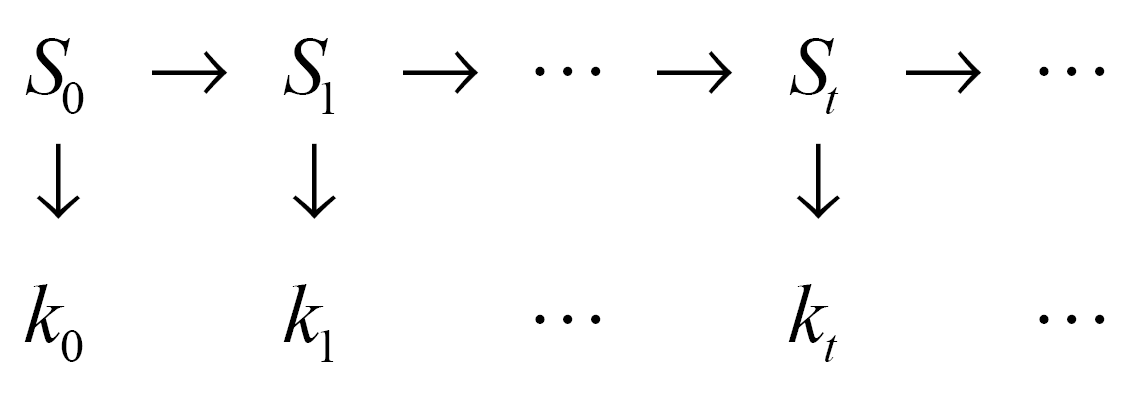
\includegraphics[width=3in]{./figures/prsgmodel.png}
	\caption{Model of pseudo-random sequence generator (PRSG)}	
	\label{fig:psrg-model}
\end{figure}

If the size of each state is $n$ bits, then the maximum number of different states would be $2^n$. As a result, we have $2^n$ different keystream bits, before the keystream starts repeating due to repeating states. The keystream bits are represented by $k_0$, $k_1$ $\ldots$, $k_{m-1}$, where $m$ = $2^{n} - 1$ (which excludes the trivial state containing all \textbf{0}'s). The goal of the attacker is to find at least one value of the internal state which occurs during the generation of the keystream. The attacker could then move the PRSG forward to generate more keystream (if the keystream is limited). The found internal state could also be used to run the PRSG backwards and find the initial state. From the initial state, finding the key is not a difficult task if the initialization algorithm and other parameters are known.\\

\textit{\textbf{Prefix of the output sequence of states.}} If the current state of the PRSG is $S_r$, then an infinite output sequence can be generated by clocking the PRSG from that state. The first $p$ bits of this output sequence is called the prefix of state $S_r$ and would be represented by the bits $k_r$, $k_{r+1}$ $\ldots$, $k_{r+p-1}$. Each of the $2^n$ possible states of the PRSG would have such output sequence and thus prefixes, which usually are unique to that particular state if $p$ is greater than or equal to $n$ \cite{biryukov2000rtc}. If the size of the prefix is less than $n$, then there would be many states which could possibly generate this prefix. For example, if the size of the state is 48 bits and we consider prefixes of size 32 bits, then the total number of states which generate this prefix is about $2^{48} \times 2^{-32}$ = $2^{16}$. If the size of the prefixes is increased to 48 bits which is also the size of the state, then there is usually just one state generating the prefix. An advantage of this property is taken in the BG attack.\\

\textit{\textbf{The attack.}} We would have two phases in the attack just as in any TMTO attack. The first phase is the precomputation phase and the second phase is the attack phase. During the precomputation phase, the attacker would randomly select $n_1$ values out of the $2^n$ values the PRSG state could have. For each of these states, the prefix is computed, and the (prefix, state) pair stored in memory. The data structure that needs to be used for storing the pairs is a hash table. More details about hash tables are provided in section ??.

During the attack phase, the attacker is assumed to have access to some part of the initial keystream. In practice, the attacker would have access to the ciphertext bits. But, we assume that the attacker knows the plaintext bits before hand by some means, and thus the keystream is calculated in the following manner, $k_i$ = $p_i \oplus c_i$, as also mentioned in chapter \ref{chapter:intro}. The attacker then selects overlapping subsequences of size $n$ from the keystream, and tries to find a match in the hash table. The first subsequence would be $k_0$, $k_1$ $\ldots$, $k_{n-1}$ corresponding to state $S_0$, the second subsequence would be $k_1$, $k_2$ $\ldots$, $k_{n}$ corresponding to state $S_1$, and so on. If such a prefix exists in the memory, then the current state is determined from the matched (prefix, state) pair.\\

\textit{\textbf{Analysis of the attack.}} Let us assume that the attacker tries $n_2$ prefixes during the attack phase, before the first hit is observed. Then, we can apply the birthday paradox here, in order to find the approximate value of $n_2$. According to the variant of the birthday paradox, explained in section \ref{sec:bday-paradox}, we have the following condition:

\begin{center}
\large{$n_1 \times n_2$ $\geq$ $2^n$}
\end{center}

Also, for sufficient number of prefixes to be available, the keystream should have a length of at least $(n_2 + n - 1)$ bits. In such a case, the attacker would have exactly $n_2$ prefixes of length $n$ each to search in the memory.


\section{Babbage-Golic attack on HiTag2}

The HiTag2 stream cipher is introduced in section \ref{sec:hitag2}. We are going to consider a variant of the BG attack to be implemented on HiTag2. The attack phase of the BG attack is going to be the same, but the precomputation phase is modified so that we have a match in the memory with certainty \cite{erik-discussions}. \\

\textit{\textbf{Precomputation phase.}} During the precomputation phase, the selection of states is not done at random now, but with certain determinism. Only an initial state is selected at random for precomputation ($S_{initial}$), while the remaining states are derived using this state. The prefix for $S_{initial}$ is first computed and the (prefix, state) pair stored in the hash table. The next state is derived using a state transition function, which returns the state $q$ states ahead of the current state. The next state then is represented by $S_{initial+q}$. Similarly, the prefix for $S_{initial+q}$ is computed and the (prefix, state) pair stored in the hash table. The process is repeated, and consequently we have a list of states (and their corresponding prefixes) in memory which are at a \emph{distance} of $q$ states from each other. These would be $S_{initial}$, $S_{initial+q}$, $S_{initial+2q}$ and so on. Until the complete circle of states is covered (after which the same states are repeated) we have unique (prefix, state) pairs stored for the precomputation phase. At the end of the precomputation phase, we would have a total of $2^n/q$ states in the hash table. The precomputation phase would take and order of $2^n/q$ of memory space.\\

\textit{\textbf{Attack phase.}} Let us assume that the initial state of the keystream available to the attacker is $S_{unknown}$ (as this state is unknown to the attacker). The attacker selects subsequences from the keystream and matches them with the prefixes stored in the memory. Then, it is our claim that if the attacker gets $q$ subsequences from the keystream (which represent $q$ unknown states), a prefix in the memory is bound to get matched with a keystream subsequence. It is because the fixed distance between any two states in the memory is that of $q$ states. Hence, in the worst case, the attack phase would take $q$ order of operations to find a match in the memory. \\

\textit{\textbf{Matrix representation of state transition function.}} As mentioned above, the state transition function is used in the precomputation phase for deriving a non-adjacent state from the current state. The design of the this function needs an important consideration, which we discuss here. The update function in LFSR can be represented by a binary matrix $U$ \cite{trappe2005icc}. The topmost row of $U$ contains \textbf{1} at positions representing the tap bits, and \textbf{0} otherwise. In the remaining rows of $U$, the values of the bits are such that the last 47 bits of the new state are the first 47 bits of the previous state. It must be noted that the indexing in the matrix is the same as that in the state register. Thus, the leftmost position in the top row of the matrix represents the \textbf{48}'th bit in the state register, and the rightmost position represents the \textbf{1}'st bit in the state register. The matrix $U$ for HiTag2 is shown in figure \ref{fig:hitag2-transition-matrix}.

\begin{figure}[h!]
	\centering
	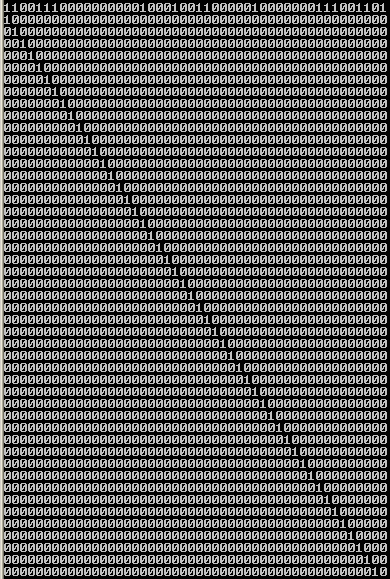
\includegraphics[width=3.5in]{./figures/hitag2-transition-matrix.png}
	\caption{Update function matrix $U$ for HiTag2}	
	\label{fig:hitag2-transition-matrix}
\end{figure}

If the current state of the LFSR is $S_{current}$, then the next state $S_{next}$ can be computed by the matrix multiplication shown below.

\begin{center}
\large{$U . S_{current}$ = $S_{next}$}\\
\end{center}

This is represented in the matrix notation as follows.

\begin{center}
\large{
$U.$
$\begin{bmatrix}
s_{n} \\
s_{n-1} \\
\vdots \\
s_{1} \\
s_{0}
\end{bmatrix}$ = 
$\begin{bmatrix}
s_{new} \\
s_{n} \\
\vdots \\
s_{2} \\
s_{1}
\end{bmatrix}$}
\end{center}

Matrix multiplication for binary matrices is to perform a bitwise boolean \emph{and} operation (denoted by \&) and then \emph{xor} the resulting bits. In notation, if we have two rows $r_1$ and $r_2$ of size $n$ for multiplication, then we have the following,

\begin{center}
\large{$r_1$ = $r_{11} r_{12} \ldots r_{1n}$}\\
\large{$r_2$ = $r_{21} r_{22} \ldots r_{2n}$}\\
\large{$r_1 \times r_2$ = $(r_{11} \& r_{21}) \oplus (r_{12} \& r_{22}) \oplus \ldots \oplus (r_{1n} \& r_{2n})$}
\end{center}

To compute the state occuring $q$ states after the current state, we perform the above matrix multiplication $q$ times, as follows,

\begin{center}
\large{$S_{current + q}$ = $\underbrace{U . U . U \dots U}_{q} . S_{current}$}, or\\
\large{$S_{current + q}$ = $U^q . S_{current}$}\\
\end{center}

The entire precomputation phase would require $2^n/q$ states. Thus, if we have to repeat the above multiplication for $2^n/q$ states, the total number of matrix multiplications required would be $2^n$, since the computation for one state requires $q$ multiplications. In the case of HiTag2, an order of $2^{48}$ operations would be required for precomputation, which would take years to complete.

From \cite{erik-discussions}, there is a better solution for computing the states for the precomputation phase. Instead of performing matrix multiplication by multiplying with $U$ each time, a repeated square of $U$ can be performed yielding an efficient algorithm. The square of $U$ is first computed, which is squared to compute $U^4$, which is again squared to compute $U^8$, and so on. If $\log_2{q}$ is an integer, then the squaring is repeated for $\log_2{q}$ number of times, as shown below.

\begin{center}
\large{$S_{current + q}$ = $(((U^2)^2) \underbrace{\dotsc}_{\log_2{q}})^2 . S_{current}$}\\
\end{center}
\label{eq:state-trans}

As can be seen, computing each state would take $\log_2{q}$ multiplications, and thus the entire precomputation phase would take $q \times \log_2{q}$ matrix multiplications. This is much effecient than the previous complexity of $2^n$. The above equation shall then be used in the precomputation phase of this attack to compute the (prefix, state) pairs.\\

\textit{\textbf{Implementation details.}}
% implementation results %
% TMD calculations, specially data requirement for the attack %

\section{Variant of Babbage-Golic attack on HiTag2}
In the previous attack, there is a big assumption on the amount of keystream available to the attacker. The requirement for the keystream is proportional to the number of operations performed during the attack phase. Considering the use of HiTag2 in car keys, it is certain that such long keystream would not be available. Rather several short keystreams (for each transaction between the car and car key) would be available to attacker over a span of time. The difference in each such keystream would be in the initial state, arising due to a different IV every time. The secret key shared between the car and the car key would be the same, and for every transaction a new random IV is generated and used in computing the initial state. 

As explained in section \ref{sec:hitag2}, 32 bits of data is exchanged between the car and the car key, when a transaction takes place. These 32 bits of data, known as the \emph{tag}, perform the function of authenticating the car key to the car. 

